\documentclass[10pt,a4paper]{article}

% --- Packages ---
\usepackage[utf8]{inputenc}
\usepackage[T1]{fontenc}
\usepackage{helvet}
\renewcommand{\familydefault}{\sfdefault}

\usepackage[margin=1.2cm,top=1.5cm,bottom=1.8cm,headheight=14pt]{geometry}
\usepackage{xcolor}

% Custom Palette (2-4 primary + functional accents)
\definecolor{PrimaryBlue}{HTML}{1E3A8A}
\definecolor{TealAccent}{HTML}{0D9488}
\definecolor{DarkText}{HTML}{1F2937}
\definecolor{LightBg}{HTML}{F8FAFC}
\definecolor{BorderGray}{HTML}{CBD5E1}
\definecolor{PassGreen}{HTML}{15803D}
\definecolor{WarnAmber}{HTML}{D97706}
\definecolor{FailRed}{HTML}{B91C1C}
\definecolor{PurpleAccent}{HTML}{6B21A8}

\usepackage{amsmath,amssymb}
\usepackage{tabularx,booktabs,colortbl,array}
\usepackage{tcolorbox}
\tcbuselibrary{skins,breakable}
\usepackage{tikz}
\usetikzlibrary{positioning,calc,shapes.geometric,backgrounds,patterns}
\usepackage{fontawesome5}
\usepackage{fancyhdr}
\usepackage{enumitem}
\usepackage{titlesec}
\usepackage{microtype}
\usepackage{lastpage}

% --- Page Setup & Headers ---
\pagestyle{fancy}
\fancyhf{}
\rhead{\small\color{DarkText}\textbf{MERIDIAN GENOMICS} \ensuremath{\cdot} High-Throughput Processing Manifest}
\lhead{\small\color{DarkText}\textbf{Doc ID:} PRJ-2026-NEX-0842}
\rfoot{\small\color{DarkText}Page \thepage\ of \pageref{LastPage}}
\lfoot{\small\color{DarkText}\faLock\ Confidential -- Meridian Core Genomics Facility}
\renewcommand{\headrulewidth}{0.4pt}
\renewcommand{\footrulewidth}{0.4pt}

% --- Section Styling ---
\titleformat{\section}
  {\color{PrimaryBlue}\normalfont\Large\bfseries}
  {\thesection}{1em}{}
  [\color{TealAccent}\titlerule]

\titleformat{\subsection}
  {\color{PrimaryBlue}\normalfont\large\bfseries}
  {\thesubsection}{0.5em}{}

\titlespacing*{\section}{0pt}{12pt}{8pt}
\titlespacing*{\subsection}{0pt}{8pt}{4pt}

% --- Helper Commands ---
\newcommand{\statusbadge}[2]{%
  \setlength{\fboxsep}{2pt}%
  \colorbox{#1!15!white}{\color{#1}\fontsize{6.5pt}{7.5pt}\selectfont\textbf{#2}}%
}

\begin{document}

% ==========================================
% HEADER BLOCK
% ==========================================
\begin{tcolorbox}[
  enhanced,
  colback=PrimaryBlue,
  colframe=PrimaryBlue,
  arc=3pt,
  left=12pt, right=12pt, top=10pt, bottom=10pt,
  coltext=white
]
  \begin{minipage}[c]{0.62\linewidth}
    {\fontsize{18pt}{22pt}\selectfont\bfseries MERIDIAN GENOMICS CORE} \\[3pt]
    {\fontsize{11pt}{14pt}\selectfont\color{TealAccent!30!white}\faDna\ High-Throughput DNA/RNA Sample Processing Manifest} \\[2pt]
    {\small\color{white!80!white}Advanced Genomics Facility \ensuremath{\cdot} Building B, Suite 400 \ensuremath{\cdot} Apex Research Park}
  \end{minipage}%
  \hfill
  \begin{minipage}[c]{0.35\linewidth}
    \begin{tcolorbox}[
      colback=white,
      colframe=BorderGray,
      arc=2pt,
      boxsep=4pt,
      coltext=DarkText,
      boxrule=0.5pt
    ]
      \fontsize{8pt}{10pt}\selectfont
      \textbf{Project ID:} PRJ-2026-NEX-0842 \\
      \textbf{Intake Date:} 2026-07-24 \\
      \textbf{Batch Status:} \statusbadge{PassGreen}{QC PASSED -- IN PREP} \\
      \textbf{Seq Platform:} NovaSeq X Plus
    \end{tcolorbox}
  \end{minipage}
\end{tcolorbox}

\vspace{-4pt}

% ==========================================
% METADATA SUMMARY TABLE
% ==========================================
\begin{tcolorbox}[
  enhanced,
  colback=LightBg,
  colframe=BorderGray,
  arc=2pt,
  boxrule=0.5pt,
  left=8pt, right=8pt, top=6pt, bottom=6pt
]
  \fontsize{8.5pt}{11pt}\selectfont
  \begin{tabularx}{\linewidth}{@{}l X l X@{}}
    \textbf{\faUser\ Principal Investigator:} & Dr. Eleanor Vance (Apex Bio) & \textbf{\faBuilding\ Submitting Org:} & Synapse Therapeutics Inc. \\
    \textbf{\faFlask\ Primary Workflow:} & Whole Genome Sequencing (WGS) & \textbf{\faTag\ Target Reads/Cell:} & 30x Human WGS / 50k scRNA \\
    \textbf{\faUser\ Lab Technician:} & Marcus Thorne, CLS & \textbf{\faCalendar\ Scheduled Run:} & 2026-07-26 (Lane 3 \& 4) \\
    \textbf{\faBarcode\ Sample Count:} & 24 Samples (1 Plate, Wells A01--C08) & \textbf{\faClipboardCheck\ QC Protocol:} & ISO/IEC 17025 Standard \\
  \end{tabularx}
\end{tcolorbox}

\vspace{4pt}

% ==========================================
% SECTION 1: INTAKE & QC CRITERIA
% ==========================================
\section{\faClipboardCheck\ Section 1: Sample Intake Checklist \& Threshold Criteria}

\begin{minipage}[t]{0.48\linewidth}
  \begin{tcolorbox}[
    title={\small\bfseries\faSlidersH\ Technical Acceptance Criteria},
    colback=white,
    colframe=PrimaryBlue,
    coltitle=white,
    arc=2pt,
    boxrule=0.5pt,
    top=4pt, bottom=4pt, left=6pt, right=6pt
  ]
    \fontsize{8pt}{10.5pt}\selectfont
    \begin{tabular}{@{}l l l@{}}
      \textbf{Parameter} & \textbf{WGS Standard} & \textbf{scRNA-Seq} \\
      \hline
      Min Concentration & $\ge 10.0$ ng/$\mu$L & $\ge 500$ cells/$\mu$L \\
      Total Input Mass & $\ge 100$ ng & $\ge 50,000$ cells \\
      Min Volume & $\ge 20\,\mu$L & $\ge 15\,\mu$L \\
      A260/A280 Ratio & $1.80 - 2.00$ & N/A \\
      A260/A230 Ratio & $2.00 - 2.20$ & N/A \\
      RIN / DIN Score & DIN $\ge 7.5$ & RIN $\ge 8.0$ \\
      Buffer Media & 10mM Tris-HCl & 1x PBS + 0.04\% BSA \\
    \end{tabular}
  \end{tcolorbox}
\end{minipage}%
\hfill
\begin{minipage}[t]{0.48\linewidth}
  \begin{tcolorbox}[
    title={\small\bfseries\faCheckCircle\ Intake Quality Assurance Log},
    colback=white,
    colframe=TealAccent,
    coltitle=white,
    arc=2pt,
    boxrule=0.5pt,
    top=4pt, bottom=4pt, left=6pt, right=6pt
  ]
    \fontsize{8pt}{10.5pt}\selectfont
    \begin{itemize}[leftmargin=12pt, itemsep=2pt, label={\color{PassGreen}\faCheck}]
      \item Sample tubes inspected for seal integrity and leakage.
      \item Barcodes scanned and matched against submission manifest.
      \item Fluorometric quantification (Qubit 4.0 BR DNA Assay).
      \item Microfluidic electrophoresis (Agilent TapeStation 4200).
      \item Cell viability assessed via automated trypan blue counting ($>92\%$).
      \item Samples aliquoted into 96-well reaction plate (Lot \#20260710).
    \end{itemize}
  \end{tcolorbox}
\end{minipage}

\par
\vspace{6pt}

% ==========================================
% SECTION 2: 96-WELL PLATE LAYOUT MAP (TIKZ)
% ==========================================
\section{\faTable\ Section 2: 96-Well Plate Batch Map (Plate Barcode: PLT-96-NEX-4412)}

\begin{tcolorbox}[
  enhanced,
  colback=LightBg,
  colframe=BorderGray,
  arc=2pt,
  boxrule=0.5pt,
  left=4pt, right=4pt, top=6pt, bottom=6pt
]
  \centering
  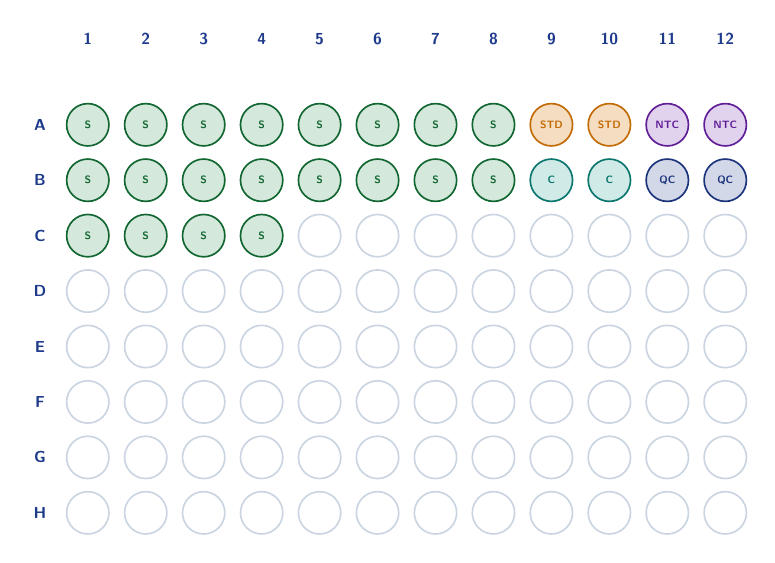
\begin{tikzpicture}[scale=0.64, transform shape]
    % Draw Grid Letters and Numbers
    \foreach \x [count=\col from 1] in {1,2,3,4,5,6,7,8,9,10,11,12} {
      \node[font=\bfseries\small, color=PrimaryBlue] at (\x*1.15, 0.6) {\col};
    }
    \foreach \y [count=\row from 1] in {A,B,C,D,E,F,G,H} {
      \node[font=\bfseries\small, color=PrimaryBlue] at (0.2, -\row*1.1) {\y};
    }

    % Define well colors helper pattern:
    \foreach \r in {1,2,3,4,5,6,7,8} {
      \foreach \col in {1,2,3,4,5,6,7,8,9,10,11,12} {
        \pgfmathsetmacro{\isGreen}{(\r==1 && \col<=8) || (\r==2 && \col<=8) || (\r==3 && \col<=4) ? 1 : 0}
        \pgfmathsetmacro{\isTeal}{(\r==2 && \col>=9 && \col<=10) ? 1 : 0}
        \pgfmathsetmacro{\isGold}{(\r==1 && \col>=9 && \col<=10) ? 1 : 0}
        \pgfmathsetmacro{\isPurple}{(\r==1 && \col>=11) ? 1 : 0}
        \pgfmathsetmacro{\isBlue}{(\r==2 && \col>=11) ? 1 : 0}

        \ifdim \isGreen pt=1 pt
          \def\wcolor{PassGreen!80!black}
          \def\wbg{PassGreen!18!white}
          \def\wtext{S}
        \else
          \ifdim \isTeal pt=1 pt
            \def\wcolor{TealAccent!80!black}
            \def\wbg{TealAccent!20!white}
            \def\wtext{C}
          \else
            \ifdim \isGold pt=1 pt
              \def\wcolor{WarnAmber!90!black}
              \def\wbg{WarnAmber!25!white}
              \def\wtext{STD}
            \else
              \ifdim \isPurple pt=1 pt
                \def\wcolor{PurpleAccent!90!black}
                \def\wbg{PurpleAccent!20!white}
                \def\wtext{NTC}
              \else
                \ifdim \isBlue pt=1 pt
                  \def\wcolor{PrimaryBlue!90!black}
                  \def\wbg{PrimaryBlue!20!white}
                  \def\wtext{QC}
                \else
                  \def\wcolor{BorderGray}
                  \def\wbg{white}
                  \def\wtext{}
                \fi
              \fi
            \fi
          \fi
        \fi

        % Draw well circle
        \draw[line width=0.6pt, color=\wcolor, fill=\wbg] (\col*1.15, -\r*1.1) circle (0.42cm);
        \ifx\wtext\empty
        \else
          \node[font=\fontsize{6pt}{6pt}\selectfont\bfseries, color=\wcolor] at (\col*1.15, -\r*1.1) {\wtext};
        \fi
      }
    }
  \end{tikzpicture}

  \vspace{4pt}
  \fontsize{7.5pt}{9.5pt}\selectfont
  \centering
  \begin{tabular}{c c c}
    \tikz\draw[line width=0.6pt, color=PassGreen!80!black, fill=PassGreen!18!white] (0,0) circle (0.15cm); \textbf{DNA Samples} (S01--S20) &
    \tikz\draw[line width=0.6pt, color=TealAccent!80!black, fill=TealAccent!20!white] (0,0) circle (0.15cm); \textbf{scRNA-Seq} (C01--C02) &
    \tikz\draw[line width=0.6pt, color=WarnAmber!90!black, fill=WarnAmber!25!white] (0,0) circle (0.15cm); \textbf{DNA Standard} (STD1--2) \\[3pt]
    \tikz\draw[line width=0.6pt, color=PurpleAccent!90!black, fill=PurpleAccent!20!white] (0,0) circle (0.15cm); \textbf{No-Template Control} &
    \tikz\draw[line width=0.6pt, color=PrimaryBlue!90!black, fill=PrimaryBlue!20!white] (0,0) circle (0.15cm); \textbf{PhiX/QC Spike} &
    \tikz\draw[line width=0.6pt, color=BorderGray, fill=white] (0,0) circle (0.15cm); \textbf{Empty Well} \\
  \end{tabular}
\end{tcolorbox}

\newpage

% ==========================================
% PAGE 2: SAMPLE MANIFEST TABLE
% ==========================================
\section{\faVial\ Section 3: High-Throughput Sample Extraction \& QC Manifest}

\fontsize{7.5pt}{9.5pt}\selectfont
\rowcolors{2}{LightBg}{white}
\begin{tabularx}{\linewidth}{@{} c l l X c c c c c c c @{}}
  \rowcolor{PrimaryBlue}
  \color{white}\textbf{Well} & \color{white}\textbf{Sample ID} & \color{white}\textbf{Client Label} & \color{white}\textbf{Tissue / Specimen} & \color{white}\textbf{Conc} & \color{white}\textbf{Vol} & \color{white}\textbf{Yield} & \color{white}\textbf{260/280} & \color{white}\textbf{260/230} & \color{white}\textbf{RIN/DIN} & \color{white}\textbf{Status} \\
  \rowcolor{PrimaryBlue}
  & & & & \color{white}(ng/$\mu$L) & \color{white}($\mu$L) & \color{white}($\mu$g) & & & & \\
  \hline
  A01 & NEX-0842-01 & PBMC-Norm-101 & Human Blood PBMC & 42.5 & 35.0 & 1.49 & 1.88 & 2.12 & DIN 8.9 & \statusbadge{PassGreen}{PASS} \\
  A02 & NEX-0842-02 & PBMC-Norm-102 & Human Blood PBMC & 38.2 & 35.0 & 1.34 & 1.86 & 2.08 & DIN 8.7 & \statusbadge{PassGreen}{PASS} \\
  A03 & NEX-0842-03 & T-Tumor-FFPE-A & FFPE Liver Carcinoma & 18.4 & 25.0 & 0.46 & 1.79 & 1.94 & DIN 6.8 & \statusbadge{WarnAmber}{WARN} \\
  A04 & NEX-0842-04 & T-Tumor-FFPE-B & FFPE Liver Carcinoma & 22.1 & 25.0 & 0.55 & 1.82 & 2.01 & DIN 7.1 & \statusbadge{PassGreen}{PASS} \\
  A05 & NEX-0842-05 & Organoid-C3-d14 & Cerebral Organoid & 54.0 & 40.0 & 2.16 & 1.91 & 2.15 & RIN 9.2 & \statusbadge{PassGreen}{PASS} \\
  A06 & NEX-0842-06 & Organoid-C3-d28 & Cerebral Organoid & 49.8 & 40.0 & 1.99 & 1.90 & 2.14 & RIN 9.0 & \statusbadge{PassGreen}{PASS} \\
  A07 & NEX-0842-07 & CSF-CellFree-01 & Cell-Free Plasma DNA & 4.2 & 50.0 & 0.21 & 1.75 & 1.82 & DIN 5.4 & \statusbadge{WarnAmber}{LOW-IN} \\
  A08 & NEX-0842-08 & CSF-CellFree-02 & Cell-Free Plasma DNA & 5.1 & 50.0 & 0.26 & 1.78 & 1.88 & DIN 5.9 & \statusbadge{WarnAmber}{LOW-IN} \\
  A09 & STD-NEX-01 & Control-gDNA-100 & Human Reference gDNA & 100.0 & 50.0 & 5.00 & 1.89 & 2.18 & DIN 9.8 & \statusbadge{PassGreen}{PASS} \\
  A10 & STD-NEX-02 & Control-gDNA-50 & Human Reference gDNA & 50.0 & 50.0 & 2.50 & 1.88 & 2.17 & DIN 9.7 & \statusbadge{PassGreen}{PASS} \\
  A11 & NTC-BLANK-1 & Buffer-Control-1 & Nuclease-Free H2O & 0.02 & 50.0 & 0.00 & -- & -- & -- & \statusbadge{PassGreen}{PASS} \\
  A12 & NTC-BLANK-2 & Buffer-Control-2 & Nuclease-Free H2O & 0.01 & 50.0 & 0.00 & -- & -- & -- & \statusbadge{PassGreen}{PASS} \\
  \hline
  B01 & NEX-0842-09 & Mouse-Brain-CTX & C57BL/6 Cortex Tissue & 68.4 & 30.0 & 2.05 & 1.92 & 2.19 & RIN 8.8 & \statusbadge{PassGreen}{PASS} \\
  B02 & NEX-0842-10 & Mouse-Brain-HIP & C57BL/6 Hippocampus & 61.2 & 30.0 & 1.84 & 1.91 & 2.16 & RIN 8.6 & \statusbadge{PassGreen}{PASS} \\
  B03 & NEX-0842-11 & CellLine-HEK293T & Cultured Cell Lysate & 112.5 & 40.0 & 4.50 & 1.94 & 2.21 & RIN 9.6 & \statusbadge{PassGreen}{PASS} \\
  B04 & NEX-0842-12 & CellLine-K562 & Cultured Cell Lysate & 108.0 & 40.0 & 4.32 & 1.93 & 2.20 & RIN 9.5 & \statusbadge{PassGreen}{PASS} \\
  B05 & NEX-0842-13 & Plant-Arabidopsis & Leaf Tissue Extract & 31.7 & 35.0 & 1.11 & 1.81 & 1.92 & DIN 7.4 & \statusbadge{PassGreen}{PASS} \\
  B06 & NEX-0842-14 & Plant-ZeaMays & Root Tip Tissue & 28.4 & 35.0 & 0.99 & 1.78 & 1.89 & DIN 7.2 & \statusbadge{PassGreen}{PASS} \\
  B07 & NEX-0842-15 & Skin-Biopsy-01 & Dermal Punch Biopsy & 15.2 & 20.0 & 0.30 & 1.84 & 1.98 & DIN 7.6 & \statusbadge{PassGreen}{PASS} \\
  B08 & NEX-0842-16 & Skin-Biopsy-02 & Dermal Punch Biopsy & 14.8 & 20.0 & 0.30 & 1.83 & 1.95 & DIN 7.6 & \statusbadge{PassGreen}{PASS} \\
  B09 & SINGLE-CELL-01 & scRNA-PBMC-Fresh & Single-Cell Suspension & -- & 20.0 & -- & -- & -- & Viab 94\% & \statusbadge{PassGreen}{PASS} \\
  B10 & SINGLE-CELL-02 & scRNA-Tumor-Single & Single-Cell Suspension & -- & 20.0 & -- & -- & -- & Viab 91\% & \statusbadge{PassGreen}{PASS} \\
  B11 & QC-SPIKE-01 & ERCC-Control-Mix & Synthetic RNA Spikes & 10.0 & 15.0 & 0.15 & 1.95 & 2.20 & Standard & \statusbadge{PassGreen}{PASS} \\
  B12 & QC-SPIKE-02 & PhiX-Library-v3 & Control Library Spike & 10.0 & 15.0 & 0.15 & -- & -- & -- & \statusbadge{PassGreen}{PASS} \\
  \hline
  C01 & NEX-0842-17 & Saliva-Swab-A1 & Buccal Epithelial Swab & 26.5 & 40.0 & 1.06 & 1.82 & 2.04 & DIN 8.1 & \statusbadge{PassGreen}{PASS} \\
  C02 & NEX-0842-18 & Saliva-Swab-A2 & Buccal Epithelial Swab & 29.1 & 40.0 & 1.16 & 1.85 & 2.07 & DIN 8.3 & \statusbadge{PassGreen}{PASS} \\
  C03 & NEX-0842-19 & Stool-Metagenome & Gut Microbiome Extract & 44.0 & 30.0 & 1.32 & 1.76 & 1.68 & DIN 6.5 & \statusbadge{WarnAmber}{LOW-230} \\
  C04 & NEX-0842-20 & Soil-Metagenome & Environmental Soil & 12.0 & 30.0 & 0.36 & 1.68 & 1.45 & DIN 5.8 & \statusbadge{FailRed}{FAIL-RE-EXT} \\
  \bottomrule
\end{tabularx}

\vspace{8pt}

% ==========================================
% SECTION 4: LIBRARY PREP & INDEXING ASSIGNMENT
% ==========================================
\section{\faBarcode\ Section 4: Library Preparation Protocol \& Dual-Index Barcode Scheme}

\begin{tcolorbox}[
  enhanced,
  colback=LightBg,
  colframe=BorderGray,
  arc=2pt,
  boxrule=0.5pt,
  top=6pt, bottom=6pt, left=8pt, right=8pt
]
  \fontsize{8pt}{10.5pt}\selectfont
  \begin{tabularx}{\linewidth}{@{}X X X X@{}}
    \textbf{Kit Name:} NEBNext Ultra II FS DNA & \textbf{Kit Lot \#:} LOT-2026-0618-A & \textbf{Index Set:} Unique Dual Index (UDI) 96 & \textbf{Index Lot \#:} UDI-SET-96-04 \\
    \textbf{Enzymatic Frag:} 12.5 min @ 37\ensuremath{^\circ}C & \textbf{Adapter Ligation:} 15 min @ 20\ensuremath{^\circ}C & \textbf{PCR Amplification:} 6 Cycles & \textbf{Bead Clean (SPRI):} 0.8x Size Select \\
  \end{tabularx}
\end{tcolorbox}

\vspace{4pt}

\rowcolors{2}{LightBg}{white}
\fontsize{7.5pt}{9.5pt}\selectfont
\begin{tabularx}{\linewidth}{@{} c l l X l X l @{}}
  \rowcolor{PrimaryBlue}
  \color{white}\textbf{Well} & \color{white}\textbf{Sample ID} & \color{white}\textbf{i7 Index ID} & \color{white}\textbf{i7 Sequence (P7)} & \color{white}\textbf{i5 Index ID} & \color{white}\textbf{i5 Sequence (P5)} & \color{white}\textbf{Target Reads} \\
  \hline
  A01 & NEX-0842-01 & UDI001\_i7 & \texttt{GATCGATC} & UDI001\_i5 & \texttt{ATCGATCG} & 40 M Paired-End \\
  A02 & NEX-0842-02 & UDI002\_i7 & \texttt{AGCTAGCT} & UDI002\_i5 & \texttt{CGATCGAT} & 40 M Paired-End \\
  A03 & NEX-0842-03 & UDI003\_i7 & \texttt{TCGATCGA} & UDI003\_i5 & \texttt{GATCGATC} & 40 M Paired-End \\
  A04 & NEX-0842-04 & UDI004\_i7 & \texttt{CTAGCTAG} & UDI004\_i5 & \texttt{AGCTAGCT} & 40 M Paired-End \\
  A05 & NEX-0842-05 & UDI005\_i7 & \texttt{GCTAGCTA} & UDI005\_i5 & \texttt{TCGATCGA} & 50 M Paired-End \\
  A06 & NEX-0842-06 & UDI006\_i7 & \texttt{TAGCTAGC} & UDI006\_i5 & \texttt{CTAGCTAG} & 50 M Paired-End \\
  B01 & NEX-0842-09 & UDI009\_i7 & \texttt{CGATCGAT} & UDI009\_i5 & \texttt{GCTAGCTA} & 40 M Paired-End \\
  B02 & NEX-0842-10 & UDI010\_i7 & \texttt{ATCGATCG} & UDI010\_i5 & \texttt{TAGCTAGC} & 40 M Paired-End \\
  B09 & SINGLE-CELL-01 & 10x-SI-TT-A1 & \texttt{GTAACATGCG} & 10x-SI-NT-A1 & \texttt{AGGTCATCGT} & 100 M scRNA \\
  B10 & SINGLE-CELL-02 & 10x-SI-TT-A2 & \texttt{GTCCATGCAT} & 10x-SI-NT-A2 & \texttt{GACTAGCTAG} & 100 M scRNA \\
  \bottomrule
\end{tabularx}

\newpage

% ==========================================
% PAGE 3: PRE-SEQUENCING QC & POOLING
% ==========================================
\section{\faLayerGroup\ Section 5: Pre-Sequencing QC \& Pool Normalization}

\begin{minipage}[t]{0.48\linewidth}
  \begin{tcolorbox}[
    title={\small\bfseries\faMicroscope\ Fragment Size Distribution (TapeStation 4200)},
    colback=white,
    colframe=PrimaryBlue,
    coltitle=white,
    arc=2pt,
    boxrule=0.5pt,
    top=4pt, bottom=4pt, left=6pt, right=6pt
  ]
    \fontsize{8pt}{10.5pt}\selectfont
    \begin{tabular}{@{}l l l@{}}
      \textbf{Library Pool ID} & \textbf{Peak Size (bp)} & \textbf{Molarity (nM)} \\
      \hline
      POOL-NEX-0842-WGS & 450 bp & 14.8 nM \\
      POOL-NEX-0842-scRNA & 520 bp & 22.1 nM \\
      POOL-NEX-STD-CTRL & 440 bp & 15.2 nM \\
      Final Sequenced Pool & 465 bp & \textbf{18.4 nM} \\
    \end{tabular}
    \vspace{4pt}

    {\color{DarkText}\textbf{Pass Criteria:} Average library peak size between 400--550 bp. Adapter dimer ($<120$ bp) must be $<1.0\%$.}
  \end{tcolorbox}
\end{minipage}%
\hfill
\begin{minipage}[t]{0.48\linewidth}
  \begin{tcolorbox}[
    title={\small\bfseries\faFlask\ Final Pooling \& PhiX Control Setup},
    colback=white,
    colframe=TealAccent,
    coltitle=white,
    arc=2pt,
    boxrule=0.5pt,
    top=4pt, bottom=4pt, left=6pt, right=6pt
  ]
    \fontsize{8pt}{10.5pt}\selectfont
    \begin{itemize}[leftmargin=12pt, itemsep=3pt]
      \item \textbf{Total Pool Volume:} $100\,\mu$L @ 10.0 nM target.
      \item \textbf{PhiX Control Spike-In:} 1.5\% (v/v) Illumina PhiX Control v3.
      \item \textbf{Denaturation Protocol:} $5\,\mu$L 0.2N NaOH for 5 min at room temp.
      \item \textbf{Neutralization:} $5\,\mu$L 200mM Tris-HCl pH 8.0.
      \item \textbf{Final Loading Conc:} 2.2 pM onto NovaSeq X Plus Reagent Cartridge.
    \end{itemize}
  \end{tcolorbox}
\end{minipage}

\par
\vspace{8pt}

% ==========================================
% SECTION 6: FLOW CELL & RUN PARAMETERS
% ==========================================
\section{\faCogs\ Section 6: Flow Cell Loading \& Sequencing Run Configuration}

\begin{tcolorbox}[
  enhanced,
  colback=LightBg,
  colframe=BorderGray,
  arc=2pt,
  boxrule=0.5pt,
  top=6pt, bottom=6pt, left=8pt, right=8pt
]
  \fontsize{8.5pt}{11.5pt}\selectfont
  \begin{tabularx}{\linewidth}{@{}l X l X@{}}
    \textbf{Sequencer Instrument:} & NovaSeq X Plus (SN: NSX-2024-884) & \textbf{Flow Cell Serial:} & LH-10k-202607-0091 \\
    \textbf{Flow Cell Type:} & 10B 300-Cycle Flow Cell & \textbf{Lane Assignment:} & Lane 3 \& Lane 4 \\
    \textbf{Read Configuration:} & Read 1: 151bp \ensuremath{\cdot} Read 2: 151bp & \textbf{Index Cycle Setup:} & Index 1 (i7): 10bp \ensuremath{\cdot} Index 2 (i5): 10bp \\
    \textbf{Primary Analysis:} & DRAGEN v4.2 On-Instrument Pipeline & \textbf{Output Path:} & {\fontsize{6.5pt}{7.5pt}\selectfont\texttt{s3://meridian-genomics-raw/20260724\_NEX0842/}} \\
  \end{tabularx}
\end{tcolorbox}

\vspace{10pt}

% ==========================================
% SECTION 7: CHAIN OF CUSTODY & SIGN-OFF
% ==========================================
\section{\faPen\ Section 7: Chain of Custody \& Authorization Sign-Off}

\begin{tcolorbox}[
  enhanced,
  colback=white,
  colframe=PrimaryBlue,
  arc=2pt,
  boxrule=0.5pt,
  left=8pt, right=8pt, top=8pt, bottom=8pt
]
  \fontsize{8.5pt}{12pt}\selectfont
  \begin{tabularx}{\linewidth}{@{}X X X@{}}
    \textbf{Sample Received By:} & \textbf{Library Prep Technician:} & \textbf{QA/QC Manager Approval:} \\[12pt]
    Signature: \underline{\hspace{4cm}} & Signature: \underline{\hspace{4cm}} & Signature: \underline{\hspace{4cm}} \\[6pt]
    Name: Marcus Thorne, CLS & Name: Dr. Elena Rostova & Name: Dr. Arthur Pendelton \\
    Date: 2026-07-24 & Date: 2026-07-25 & Date: 2026-07-25 \\
  \end{tabularx}

  \vspace{8pt}
  \color{DarkText}\hrule height 0.4pt
  \vspace{6pt}

  \fontsize{8pt}{10.5pt}\selectfont
  \textbf{\faInfoCircle\ Storage \& Archive Disposition:}
  \begin{itemize}[leftmargin=12pt, itemsep=1pt]
    \item Remaining stock DNA/RNA stored at \textbf{-80\ensuremath{^\circ}C Freezer \#4, Rack B, Box 12}.
    \item Constructed libraries archived at \textbf{-20\ensuremath{^\circ}C Post-PCR Library Vault 2}.
    \item Sample retention policy: Standard 6-month hold post-delivery unless extended by PI agreement.
  \end{itemize}
\end{tcolorbox}

\end{document}
